\documentclass{book}
\usepackage{graphicx}
\usepackage{fontspec}
\usepackage[utf8]{inputenc}
\usepackage[polish]{babel}
\usepackage[OT4]{polski}
\setmainfont{Latin Modern Roman}
\usepackage{hyperref}
\usepackage{geometry}
\usepackage{listings}
\usepackage{lscape}
\usepackage{csquotes}
\usepackage{graphicx}
\usepackage{caption} 
\usepackage{amsmath}
\usepackage{amsfonts}
\usepackage{array}
\usepackage{tikz}
\usetikzlibrary{shapes}
\usetikzlibrary{positioning}
\usetikzlibrary{calc}
\usetikzlibrary{fit}
\usetikzlibrary{arrows}
\usetikzlibrary{backgrounds}
\usepackage[backend=biber, bibencoding=utf8, style=numeric]{biblatex}
\addbibresource{bibliography.bib}
\graphicspath{{assets/images/}{../docs/architecture/diagrams/assets/}{../data/bak_dagster_storage/}}
\lstset{
  basicstyle=\ttfamily\small,
  breaklines=true,
  columns=fullflexible,
  keepspaces=true,
  frame=single
}

\DefineBibliographyStrings{polish}{pages = {strony}}



\begin{document}

\begin{titlepage}
\begin{center}

\vspace{72pt}

\textbf{Wyszukiwanie informacji o kościołach parafialnych z wykorzystaniem dużych modeli wizyjnych (Vision LLMs)}

\vspace{168pt}
\end{center}

\vspace{60pt}

\end{titlepage}

\tableofcontents

%Struktura głównego atrykułu, my jesteśy odpowiedzialni za częśc "%Zastosowane narzędzia - podejmowane próby i metoda wybrana na koniec - A. Podsiadły
%%Opis pakietu danych badawczych dokumentujących projekt - A. Podsiadły", przy czym nalezaloby sie skupic na razie na pierwszym punkcie

%Dotychczasowe próby wykorzystania do podobnych prac - S. Kozyra z pomocą P. Kulickiego / P. Garbacza
%Opis projektu “Podziały terytorialne” - M. Słoń
%Schematyzmy jako źródło: formularz, zróżnicowanie, stan zachowania, wiarygodność - E. Chomentowska
%Opis projektu IDUB AI - założenia, pytania badawcze - M. Słoń
%Zastosowane narzędzia - podejmowane próby i metoda wybrana na koniec - A. Podsiadły
%Opis pakietu danych badawczych dokumentujących projekt - A. Podsiadły
%Identyfikacja numeru strony i dekanatu - M. Słoń
%Identyfikacja parafii - R. Kozyrski
%Identyfikacja wezwań - E. Chomentowska
%Informacje o materiale budowlanym - J. Kumor-Mielnik
%Próby z innymi polami bazy (strona, dekanat) - M. Słoń
%Próby z innymi rodzajami źródeł (księga uposażeń, kontrybucji, wizytacja) - M. Słoń
%Podsumowanie: użyteczność narzędzia pracy dokumentacyjnej - M. Słoń
%Podsumowanie ogólne: AI w humanistyce - P. Kulicki / P. Garbacz
%
%
%Ad. 2.
%
%Od 2022 r. na KUL jest realizowany projekt „Podziały terytorialne Kościoła łacińskiego w Rzeczypospolitej (X-XXI w.). Od
%harmonizacji danych do syntezy”. Ich eksploracja zaczęła niejako od dołu, od najniższego szczebla – parafii, a chronologicznie wręcz przeciwnie, od góry, od XX w. I oczywiście fundamentem były źródła, z których należało pozyskać określone kategorie informacji i wprowadzić je do bazy danych.
%
%Ad. 3
%Dla XX i XIX w. podstawowym materiałem są schematyzmy diecezjalne. Zawierają one listę parafii i zestaw wiadomości o nich. W tych najnowszych był to względnie szeroki obraz, obejmujący między innymi materiał budowlany kościoła i jego wezwanie. W tych starszych, np. z połowy XIX w., lista ograniczała się często do samej nazwy i przyporządkowywał do jednostki wyższego rzędu, czyli dekanatu.
%Źródłami historycznymi, które autorzy projektu uznali za podstawowe dla okresów, stały się schematyzmy diecezjalne o ile zostały one sporządzone dla ustalonych przekrojów chronologicznych. One też znalazły się w zainteresowaniu autorów projektu do oceny użyteczności AI w opracowaniu tego rodzaju materiałów historycznych.
%Schematyzmy zarówno diecezjalne, jak i zakonne porównać można do drukowanych informatorów instytucjonalnych popularnych głównie pod koniec XX i na początku XXI wieku. Mają one przede wszystkim pomóc czytelnikowi w zapoznaniu się ze strukturą organizacyjną oraz obsadą osobową stanowisk w danej jednostce administracji kościelnej – czyli w omawianym przypadku poszczególnych diecezji. Schematyzmy diecezjalne zawierają również podstawowe dane personalne duchowieństwa diecezjalnego, a z czasem też wykazy osobowe męskich i żeńskich zakonów oraz zgromadzeń zakonnych. Schematyzmy (znane też pod nazwami łacińskimi takimi jak: catalogus, consignatio, elenchus, schematismus, series), w przeciwieństwie do schematyzmów zakonnych wywodzić je można od dodatków informacyjnych, które zaczęły się pojawiać przy kalendarzach liturgicznych. Te ostatnie (określane po łacinie też jako directio, directorium, kalendarium, ordo czy rubricella), to w Kościele katolickim wydawnictwa, publikowane zazwyczaj jako rocznik, które zawierają szczegółowe wskazówki dotyczące odmawiania brewiarza oraz odprawiania Mszy św. w ciągu całego roku liturgicznego. Wraz z rozwojem druku, głównie od XVIII w. zaczęto poszerzać zakres ich treści o dodatkowe wiadomości, takie jak spisy kanoników kapituł metropolitalnych, wykazy zmarłych kapłanów (który pełnił obok roli informacyjnej również dewocyjno-liturgiczną wiążącą się z obowiązkiem odprawiania Mszy Św. w intencji zmarłych[1]). Taki układ zachował się zazwyczaj do początku XIX w. Z czasem, a zwłaszcza od drugiej połowy XIX w. poszerzano treść druków, a ich układ pozwala wyodrębnić kilka zasadniczych części, które są charakterystyczne dla znacznej części roczników bez względu przynależność diecezjalną.
%W pierwszej części zamieszczano informacje o biskupach, wszystkich urzędach i stanowiskach w kurii biskupiej, organach sądowych, szkolnych itp. wraz z nazwiskami osób je piastujących. Druga istotna część elenchusów to spis parafii i duchownych pełniących w nich posługę. Tutaj również w zależności od okresu, dla którego powstawały. W połowie XIX w. mogła to być tylko nazwa miejscowości oraz nazwiska duchownych (ewentualnie z rokiem urodzenia i przyjęcia święceń kapłańskich), ale już od lat sześćdziesiątych – siedemdziesiątych XIX w. już rozszerzony wykaz informacji. Było to m.in.: wezwanie świątyni parafialnej, jej historia oraz historia parafii od daty erygowania po dość dokładne opisy historyczne zawierające najważniejsze wydarzenia z ich dziejów), patronat, liczba wiernych, terminy odpustów, wykaz miejscowości jej podległych wraz z określeniem budynku sakralnego (kościół filialny, kościół zakonny, kaplica itp.), jeśli istniał, funkcjonujących bractw, organizacji dobroczynnych czy prowadzonych dzieł, jak szkoły, przytułki czy szpitale. Poszerzeniu uległ też katalog danych dotyczących duchownych, co szczególnie istotne zdaje się w odniesieniu do proboszczów i wikariuszy. Podawany był już nie tylko rok, ale data urodzenia, święceń, objęcia placówki, zajmowane urzędy, w tym na szczeblu diecezjalnym, czy funkcje honorowe w Kościele. Osobny wykaz dotyczył duchowieństwa zakonnego: domów zakonnych zarówno męskich, jak i i żeńskich na terenie diecezji i ich mieszkańców. Zazwyczaj na końcu schematyzmu podawano nazwiska zmarłych duchownych i konsekrowanych oraz inne informacje dodatkowe. Istotnym elementem były wykazy duchownych, które ułatwiają korzystanie czytelnikowi z danego rocznika.
%Jak wspomniano, zakres i szczegółowość zawartych w elenchusach wiadomości zależała od kilku czynników: czasu powstania, autora, przyjętych w dłuższym okresie czasu rozwiązaniach w danej diecezji. Istotny wpływ na ten rodzaj druków miała również sytuacja Kościoła katolickiego w Polsce na przestrzeni ponad dwóch stuleci. Pamiętać bowiem należy, że również i on został dotknięty represjami podczas zaborów, różny był stan diecezji po odzyskaniu przez Rzeczpospolitą niepodległości, a w czasie i po drugiej wojnie światowej reżim hitlerowski i komunistyczny też wywarły piętno na działalności Kościoła, w tym też publikacji schematyzmów. Pomimo starań, by wydawać je regularnie, nie zawsze było to możliwe. Na przykład dla zaboru rosyjskiego zakazy wprowadzone po stłumieniu powstania styczniowego objęły również druk katalogów diecezjalnych. Dopiero w latach siedemdziesiątych i osiemdziesiątych XIX w. zaczęto je rozluźniać pozwalając na ich wznowienie, ale często jedynie w języku rosyjskim. Rosnąca w Polsce popularność schematyzmów i rozwój badań nad nimi o charakterze przyczynkarskim pozwala stwierdzić, iż wiedza o ich zasobach jest coraz pełniejsza. Rzadko wszystkie druki konkretnej jednostki administracyjnej przechowywane są w jednej bibliotece czy archiwum, ale w wielu przypadkach można już zidentyfikować większość tytułów. Istniejące braki często nadal wymagają odpowiedzi, co jest ich powodem. Zważywszy, iż założeniem miało być wydawanie ich co roku odnośnie brakujących roczników rodzi się pytanie czy były one wydawane i żaden z egzemplarzy nie zachował się czy też w danym roku nie ukazał się.
%Istniejące przerwy chronologiczne nie umniejszają jednak roli elenchusów w badaniach naukowych. Zawarte w nich dane o charakterze informacyjno-statystycznym bardzo często są istotną pomocą dla historii Kościoła w Polsce i jego poszczególnych diecezji, zwłaszcza w badaniach na skalę masową czy globalną dotyczącą interesującego badaczy zagadnienia. Zawdzięczają to swojej stosunkowo jednolitej formie oraz powszechności – obejmującej wszystkie diecezje polskie, chociaż w różnym stopniu i szczegółowości. W niektórych przypadkach stanowią one jedyne lub jedno z nielicznych zachowanych źródeł do poznania historii danej diecezji z określonego czasu (jak na przykład diecezja pińska[2]), jeżeli inne dokumenty uległy rozproszeniu, zaginęły lub zostały zniszczone w kolejnych pożogach wojennych.
%Wydaje się, że powyższe argumenty pozwalają zrównoważyć dwa zasadnicze braki schematyzmów: przedstawionej powyżej ich niekompletność oraz braku rzetelności danych w niektórych przypadkach. Dotyczyć mogą one różnego stopnia dokładności ich sporządzania, a tym samym występowaniu literówek, błędów w zapisie nazw miejscowości czy nazwisk, ale błędnych danych (jak wezwanie, nieaktualne nazwisko proboszcza, różnice w faktografii w historii parafii) lub powtarzania ich przez kolejne lata. Ten ostatni przykład jest szczególnie widoczny przy liczbie wiernych, która mogła nie być zmieniana kilka lat pod rząd. Nie musiał on wynikać z niedokładności autora – równie dobrze powodem mógł być brak bieżących danych lub przekazanie tej samej liczby po raz kolejny przez proboszcza danej parafii. Pomimo, iż różna może być skala i liczba takich różnic, warto pamiętać, iż schematyzmy wykorzystywane przez badacza powinny zostać poddane krytyce jak każde inne źródło historyczne, co pozwala zminimalizować ewentualne omyłki, a następnie błędy w prowadzonych analizach.
%[bibliografia wszystkich wykorzystanych roczników, bibliografia i przypisy]
%Ad. 4
%Wprowadzanie danych odbywało się w głównej mierze ręcznie, choć przy wsparciu aplikacji INDXR i z wykorzystaniem elementów oprogramowania GIS. Była to praca żmudna, angażująca kilka osób w pełnym wymiarze godzin przez kilka lat. Dla trzech przedziałów czasowych zostały wykorzystane po dwa schematyzmy dla każdej diecezji. Łącznie dało to ok. 35 000 rekordów w modelu źródłowym bazy danych.
%Lata 2022-2025 były jednocześnie okresem szybkiego wzrostu efektywności wielu narzędzi cyfrowych z AI na czele. Rozwinęły się na tyle, że stanęło pytanie o ich użyteczność w tej pracy dokumentacyjnej. Tak narodził się pomysł małej inicjatywy o nazwie “Zastosowanie zaawansowanych narzędzi cyfrowych w pracach dokumentacyjnych z zakresu geografii historycznej Kościoła”. Jego budżet był ponad stukrotnie niższy niż główny projekt i stanowił w istocie niewielki dodatek do tamtego przedsięwzięcia. Proces ekstrakcji danych miał już dobrze ugruntowaną metodę i zmierzał do końca. Ponadto droga od ogólnego pomysłu do uzyskania finansowania i uruchomienia wszystkich procedur trwała kolejne miesiące.
%Ta relacja czasowa między dwoma projektami odcisnęła swoje piętno na tym zdecydowanie mniejszym i późniejszym, który musiał być dostosowany do przedsięwzięcia w większej skali. Paradoksalnie doprowadziło to do tego, że nie tyle narzędzie wsparło prace dokumentacyjne, co te ostatnie, już wykonane, stały się podstawą dla wypracowania i przede wszystkim weryfikacji cyfrowego instrumentarium.
%Pierwszym etapem było przedstawienie informatykowi zadania merytorycznego, jakie wykonał już zespół historyków. Jednocześnie on wskazywał na ograniczenia dostępnych narzędzi. Wynikiem tego dialogu było określenie zasobu informacji, jaki ma być przedmiotem testu. Objęciem nim wszystkich pól bazy, jakie zostały uwzględnione w projekcie, uznaliśmy za niewskazane. Większość z nich rzadko pojawia się w schematyzmach i nie przyniosłyby zasobu informacji potrzebnego do oceny efektywności metody. Wynikiem automatycznej ekstrakcji miało być wypełnienie pięciu pól: numer strony źródłowej, nazwa dekanatu, nazwa parafii, wezwanie kościoła i typ jego materiału budowlanego. Każde z nich niosło ze sobą inne wyzwania.
%
%Ad. 7
%Numer strony wydawał się rzeczą najprostszą. Gdy jednak podejmowaliśmy pierwsze próby polegające na prostym prompcie, ogólnodostępnym czacie i pliku pdf o objętości kilkudziesięciu stron, właśnie tu było najwięcej błędów. Rzetelna dokumentacja wyników była jednym z fundamentów głównego projektu. To konieczne było uzyskanie poprawności bliskiej 100%. Zostało więc przyjęte takie rozwiązanie, że program analizuje oddzielnie zawartość każdej strony, a nie cały tekst źródła. Materiał pozyskany z niej był podsumowywany i jako kontekst udostępniany przy analizie kolejnej strony. Skomplikowało to bardzo treść promptu systemowego dla pola dekanat i nie okazało się w pełni skuteczne. W schematyzmie diecezji gnieźnieńskiej z 1870 r. w prawym dolnym rogu strony zapowiadano pierwszy wpis kolejnej podanie drobnym drukiem nazwy parafii. Algorytm uznał to za rozpoczęcie opisu i w automatycznym odczycie numer strony dla pierwszej parafii na danej karcie zawsze był przesunięty o jeden do tyłu. Taka forma schematyzmów jest jednak bardzo rzadka i sama pomyłka na tyle drobna, że ogólnie przyjętą metodę należy uznać z tej strony za pozytywną: odsetek błędów jest bardzo niski, przewidywalny, ograniczony do konkretnych skanów i najmniejszy z możliwych, a do tego łatwy do ręcznego skorygowania.
%Ta ostatnia cecha dotyczy również kolejnego pola - przyporządkowania parafii do dekanatów. Według nich były ułożone listy. Każdy kolejny rozdział rozpoczynał się wyróżnioną graficznie nazwą dekanatu. Nie była ona jednak powtarzana ani w żywej paginie, ani w żaden inny sposób. Informacja o przynależności dekanalnej nie była więc nigdy widoczna w samej zapisce na temat danej parafii i rzadko na stronie, gdzie ów opis się znajdował. Wybór metody analizy za każdym razem osobnej strony oznaczał więc, że dane na ten temat musiałby być jednoznacznie zapisane w podsumowaniu strony i dalej konsekwentnie dziedziczone na kolejnych, aż po zmianę. Ten skomplikowany mechanizm często działał, jednak skala błędów we wszystkich uzyskanych wynikach jest tak duża, że na tym etapie prac wyklucza użyteczność narzędzia. Jednocześnie uzupełnienie tych danych ręcznie, przy zachowaniu kolejności wpisów, jest proste i szybkie. Ten wynik jest o tyle istotny, że pokazuje ograniczone zastosowanie narzędzi AI nie tyle do oznaczania przynależności dekanalnej w schematyzmach, co do ekstrakcji danych zapisanych w podobny sposób, czyli jako tytuł wydzielonej części źródła.
%



\chapter{Zastosowane narzędzia i metoda ekstrakcji danych}\label{ch3_metoda}
\chaptermark{Metoda ekstrakcji danych}

\section{Charakterystyka zadania}\label{sec:charakterystyka_zadania}

Automatyczna ekstrakcja ustrukturyzowanych danych ze zdigitalizowanych schematyzmów diecezjalnych wpisuje się w klasę problemów określaną w informatyce jako \textit{visual document understanding} (VDU) - zagadnień, w których system komputerowy musi interpretować treść semantyczną obrazów dokumentów, uwzględniając zarówno układ typograficzny, jak i treść językową \parencite{mathew2021docvqa,jaume2019funsd}.
W odróżnieniu od generycznego rozpoznawania pisma (OCR), którego celem jest wierne przepisanie ciągłego tekstu, opisywane tu zadanie wymaga od systemu identyfikacji i klasyfikacji konkretnych \textit{pól informacyjnych} osadzonych w hierarchicznej strukturze administracyjnej, a następnie zwrócenia ich w postaci rekordów nadających się bezpośrednio do zasilenia bazy danych.

Zadanie wykazuje jednak własność, która wykracza poza standardowe problemy VDU i którą można określić mianem \textit{zależności od kontekstu międzystronicowego} (\textit{cross-page context dependency}): poprawna wartość pewnych pól na stronie~$p$ jest zdeterminowana przez informację widoczną wyłącznie na wcześniejszych stronach $1, \ldots, p-1$, nieobecną na aktualnie przetwarzanej stronie.
Standardowe benchmarki VDU takie jak DocVQA czy FUNSD przyjmują w swoich założeniach, że cała informacja niezbędna do ekstrakcji danego pola jest widoczna na tej samej stronie \parencite{mathew2021docvqa,jaume2019funsd}.
% tutaj napisac ze nasz problem wychodzi poza ramy i te benchmarki nie bylylby wystarczajace
Strukturalnie opisywana własność polega na odnajdywaniu odniesień w poprzedzającym tekście: rekord parafialny na stronie~$p$ odsyła do nagłówka dekanatu pełniącego rolę znacznika, który mógł pojawić się wiele stron wcześniej.
W odróżnieniu jednak od zagadnień \textit{long document understanding}, w których rozszerza się okno kontekstu modelu, aby objął cały dokument jednocześnie, opisywane tu rozwiązanie opiera się na selektywnej propagacji skondensowanego stanu między kolejno przetwarzanymi stronami, co czyni je bliższym sekwencyjnemu przetwarzaniu ze stanem (\textit{stateful sequential processing}) niż jednoprzebiegowemu odczytowi długiego dokumentu \parencite{beltagy2020longformer,liu2023lostmiddlelanguagemodels}.

Na każdej stronie schematyzmu może znajdować się jeden lub kilka opisów parafii, zgrupowanych pod nagłówkami dekanatów, które odpowiadają trójpoziomowej hierarchii Diecezja $\rightarrow$ Dekanat $\rightarrow$ Parafia.
Przedmiotem ekstrakcji jest pięć pól dla każdego rekordu parafialnego: (1) numer strony w druku źródłowym; (2) przynależność dekanalną; (3) nazwę parafii: (4) wezwanie kościoła; oraz (5) materiał budowlany obiektu.

Dodatkowe wyzwania wynikają ze specyfiki materiału źródłowego.
Dokumenty zostały sporządzone po łacinie z powszechnym użyciem skrótów, których dla pierwszego etapu ekstrakcji, historyczna forma musi zostać zachowana w danych wyjściowych bez jakichkolwiek zmian (np. \textit{S. Martini E.C.}, \textit{B.M.V.}, \textit{mur.}, \textit{ligna.}).

Niezależnie od wierności wobec tekstu źródłowego, system musi radzić sobie także z dużym zróżnicowaniem jakości skanów.
Mimo dobrze przeprowadzonemu procesowi digitalizacji, wiele wydań z dwudziestolecia międzywojennego współistniejących w korpusie danych z zniszczonymi woluminami z połowy XIX wieku, charakteryzuje się nieregularnym składem, plamami i wypłowiałym atramentem.
Z kolei sam układ stron waha się od pojedynczej kolumny narracyjnych opisów po gęste, dwukolumnowe zestawienia tabelaryczne, a adnotacje marginalne muszą być niezawodnie odróżniane od treści głównej.
Zestawienie dwóch reprezentatywnych przykładów takiego zróżnicowania pokazano na rys.~\ref{fig:digitalized-books-condition}.

\begin{figure}[htbp]
\centering
\begin{minipage}[t]{0.48\textwidth}
\centering
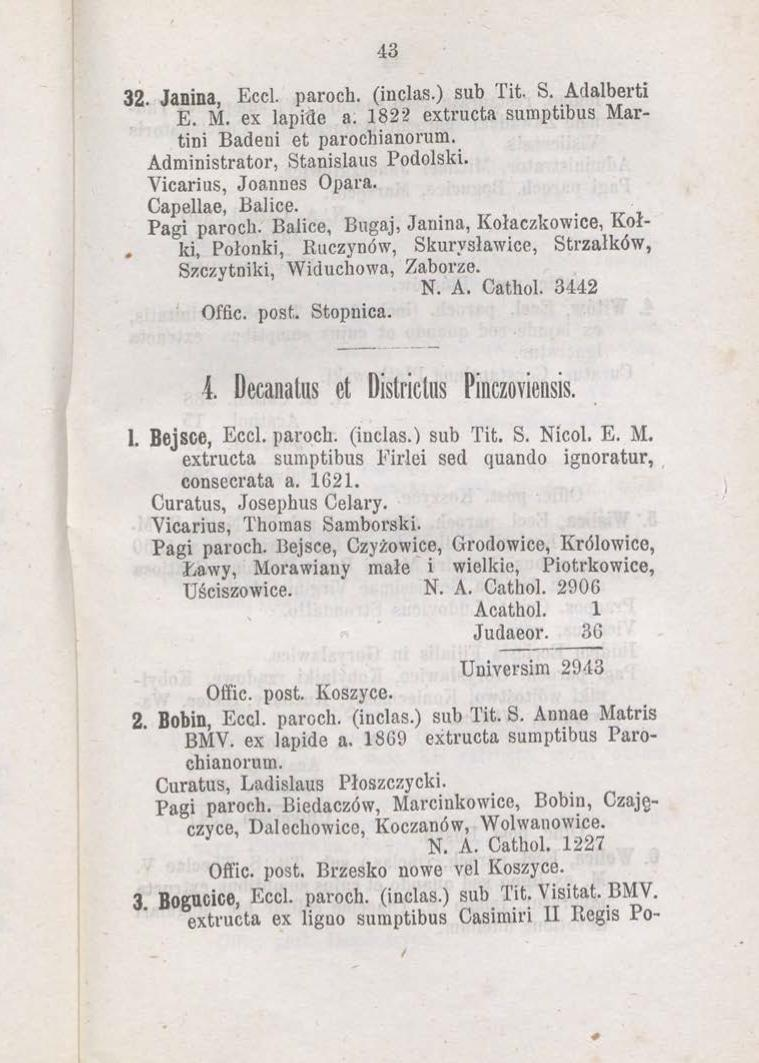
\includegraphics[width=\textwidth,height=0.34\textheight,keepaspectratio]{kielce_1874_0000c43.jpg}
\end{minipage}
\hfill
\begin{minipage}[t]{0.48\textwidth}
\centering
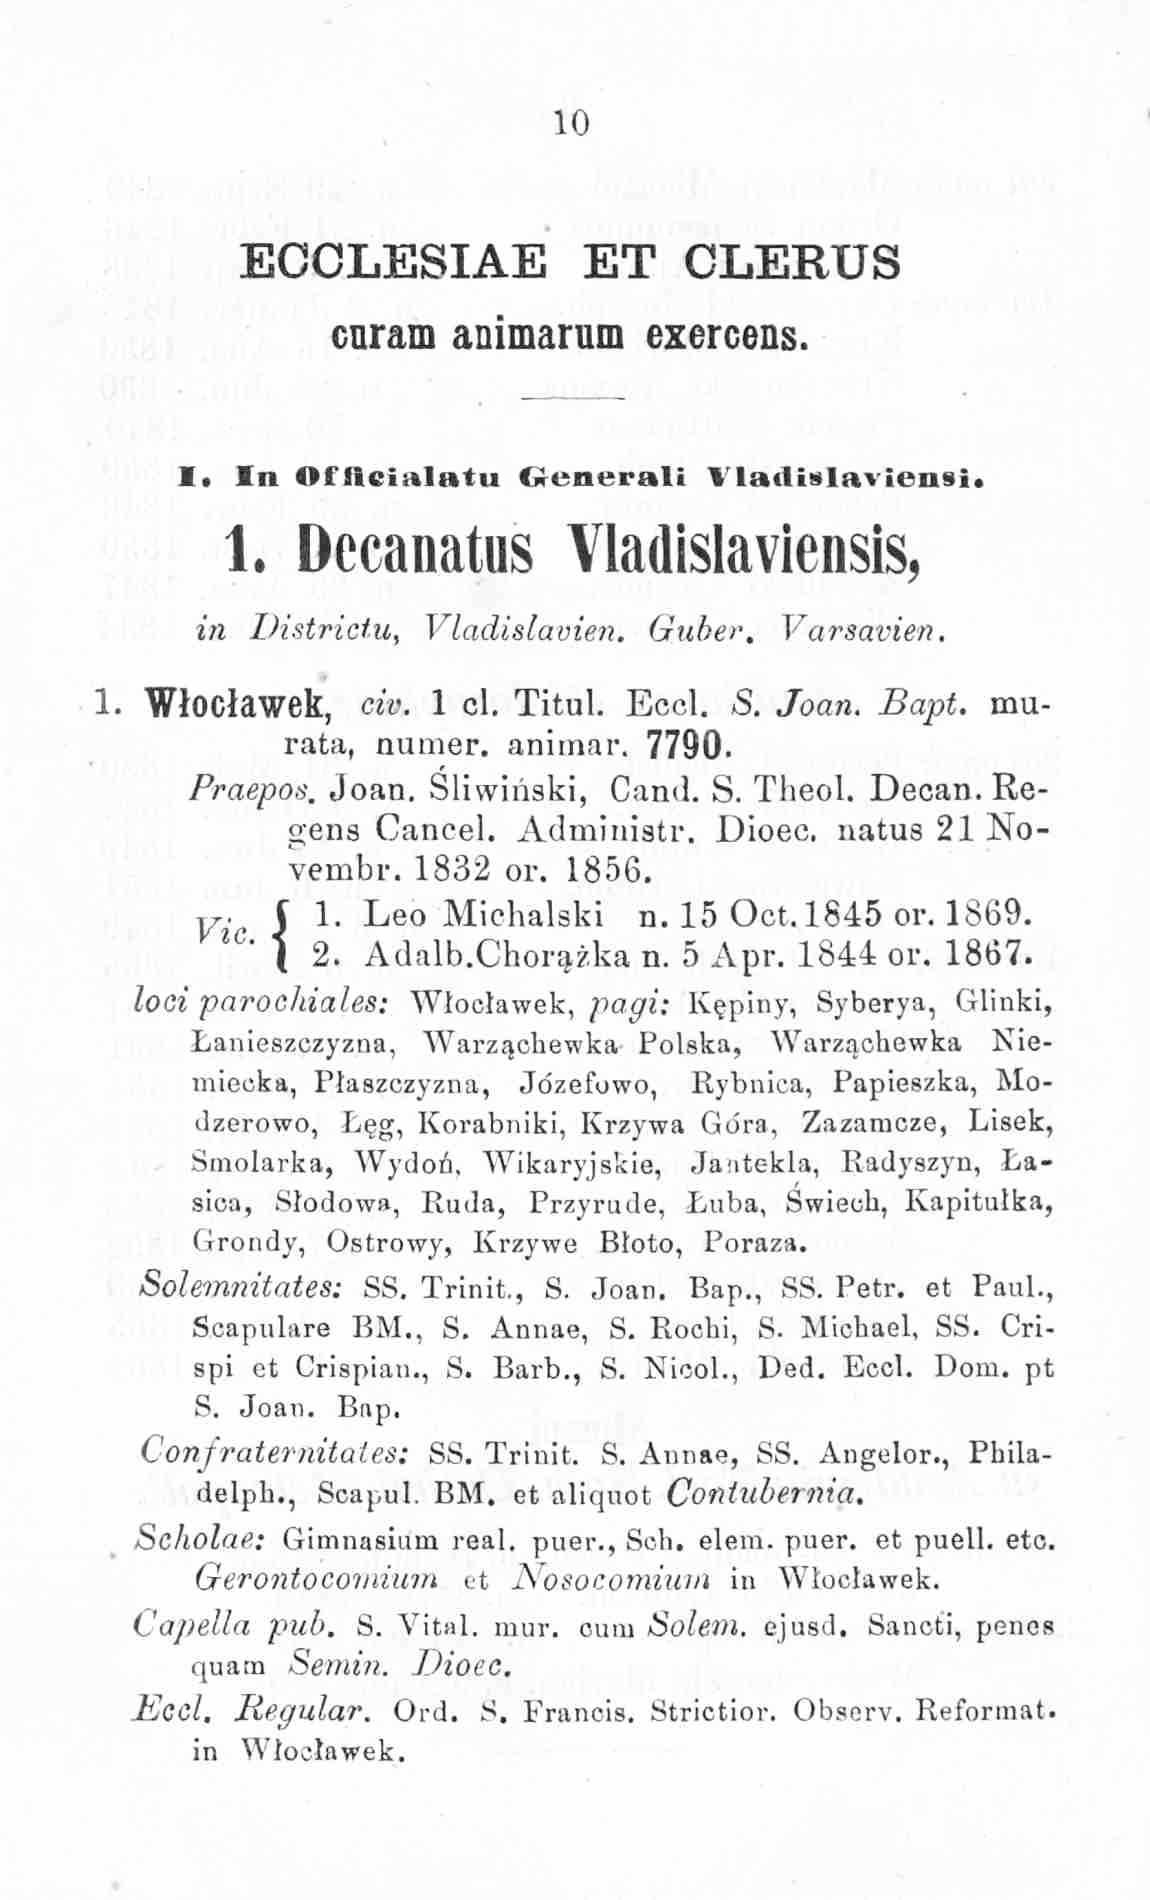
\includegraphics[width=\textwidth,height=0.34\textheight,keepaspectratio]{wloclawek_1872_0010.jpg}
\end{minipage}
\caption{Dwa przykładowe układy i stany zachowania stron schematyzmów wykorzystanych w badaniu. Po lewej widoczna jest karta o słabszej jakości i bardziej nieregularnym składzie, po prawej strona czytelniejsza, otwierająca nową sekcję dekanalną.}
\label{fig:digitalized-books-condition}
\end{figure}

Wszystkie te cechy czynią z opisywanego zadania wymagający przypadek ekstrakcji informacji z dokumentów na poziomie całego dokumentu, stosowanej w specjalistycznej domenie historycznej.

\section{Zastosowane narzędzia: podejmowane próby i wybrana metoda}\label{sec:narzedzia_metoda}

Prace nad automatyczną ekstrakcją danych ze schematyzmów nie przebiegały liniowo.
Kolejne podejścia wynikały z rozpoznania ograniczeń poprzednich metod: od prób deterministycznych, przez eksperymenty z gotowymi interfejsami modeli, po własny potok przetwarzania oparty na sekwencyjnym wywoływaniu modelu wielomodalnego.

\subsection{Metody regułowe i heurystyczne}\label{subsec:metody_regulowe}

Pierwsze eksperymenty miały charakter klasyczny: punktem wyjścia był tekst OCR, na którym próbowano budować ekstrakcję z użyciem wyrażeń regularnych, podziału na wiersze, prostych heurystyk interpunkcyjnych oraz reguł rozpoznających nagłówki i skróty.
Podejście to było atrakcyjne z inżynierskiego punktu widzenia, ponieważ dawało pełną kontrolę nad każdym etapem przetwarzania i nie wymagało kosztownych wywołań modeli generatywnych.
W praktyce okazało się jednak zbyt kruche.
Schematyzmy różniły się nie tylko językiem i zasobem skrótów, ale również liczbą kolumn, szerokością łamu, sposobem zapisu nagłówków dekanalnych oraz długością pojedynczych wpisów parafialnych.
Reguły działające poprawnie dla jednego typu układu bardzo szybko zawodziły po przejściu do innego rocznika lub diecezji, dlatego rozwiązanie to uznano za niewystarczające jako podstawa całego systemu.
Schemat ideowy tego etapu pokazuje rys.~\ref{fig:regex-approach}.

\begin{figure}[htbp]
\centering
\begin{tikzpicture}[
    >=latex,
    node distance=0.6cm and 0.6cm,
    every node/.style={font=\footnotesize},
    block/.style={draw, rounded corners, fill=gray!10, text width=2.5cm, minimum height=1.5cm, align=center},
    issue/.style={draw, rounded corners, dashed, fill=red!8, text width=4.3cm, minimum height=1.2cm, align=center}
]
\node[block] (scan) {Skan strony};
\node[block, right=of scan] (ocr) {OCR tekstowy};
\node[block, right=of ocr] (rules) {Regex i heurystyki};
\node[block, right=of rules] (output) {Rekordy pól};
\node[issue, below=0.9cm of ocr, xshift=3.1cm] (issue) {Silna zależność od konkretnego układu strony i szybka utrata skuteczności przy zmianie formatu schematyzmu.};
\draw[->, thick] (scan) -- (ocr);
\draw[->, thick] (ocr) -- (rules);
\draw[->, thick] (rules) -- (output);
\draw[->, thick] (rules) -- (issue);
\end{tikzpicture}
\caption{Podejście regułowe: ekstrakcja oparta na OCR i zestawie ręcznie definiowanych heurystyk.}
\label{fig:regex-approach}
\end{figure}

\subsection{Naiwne użycie gotowego interfejsu LLM}\label{subsec:proby_calodokumentowe}

Kolejnym krokiem było sprawdzenie, czy zadanie da się rozwiązać szybciej przy użyciu gotowego interfejsu czatowego dużego modelu językowego lub wizyjnego.
W tym wariancie do modelu przesyłano cały plik PDF schematyzmu albo pojedynczy obraz wraz z prostym poleceniem wyodrębnienia danych parafialnych.
Takie rozwiązanie miało wartość rozpoznawczą: pozwalało szybko ocenić, czy współczesne modele w ogóle potrafią zidentyfikować interesujące nas pola.
Wyniki okazały się jednak niestabilne jakościowo.
Model traktował dokument jako jednolity strumień treści, słabo zachowywał odniesienie do fizycznych stron źródła i często błędnie przypisywał numer strony do wyodrębnionych parafii.
Dodatkowym ograniczeniem był brak kontroli nad formatem odpowiedzi oraz limity długości plików i odpowiedzi narzucane przez gotowy interfejs.
Ogólny schemat tego etapu przedstawia rys.~\ref{fig:naive-llm-approach}.

\begin{figure}[htbp]
\centering
\begin{tikzpicture}[
    >=latex,
    node distance=0.6cm and 0.6cm,
    every node/.style={font=\footnotesize},
    block/.style={draw, rounded corners, fill=gray!10, text width=2.5cm, minimum height=1.5cm, align=center},
    issue/.style={draw, rounded corners, dashed, fill=red!8, text width=4.3cm, minimum height=1.2cm, align=center}
]
\node[block] (pdf) {Pełny PDF lub obraz};
\node[block, right=of pdf] (prompt) {Prosty prompt};
\node[block, right=of prompt] (chat) {Gotowy interfejs LLM};
\node[block, right=of chat] (answer) {Odpowiedź tekstowa};
\node[issue, below=0.9cm of prompt, xshift=3.1cm] (issue) {Brak kontroli nad strukturą odpowiedzi, limity interfejsu i niestabilne przypisywanie numerów stron.};
\draw[->, thick] (pdf) -- (prompt);
\draw[->, thick] (prompt) -- (chat);
\draw[->, thick] (chat) -- (answer);
\draw[->, thick] (chat) -- (issue);
\end{tikzpicture}
\caption{Naiwne użycie modelu w gotowym interfejsie czatowym.}
\label{fig:naive-llm-approach}
\end{figure}

\subsection{Próba z modelem dokumentowym LayoutLMv3}\label{subsec:layoutlmv3_attempt}

Równolegle podjęto próbę budowy bardziej klasycznego rozwiązania uczenia maszynowego, opartego na modelu LayoutLMv3 firmy Microsoft, wyspecjalizowanym w rozumieniu układu dokumentów \parencite{huang2022layoutlmv3}.
Model ten trenowano na ręcznie anotowanych stronach w notacji BIO (\textit{Beginning--Inside--Outside}), standardowo stosowanej w zadaniach rozpoznawania encji nazewniczych.
W tym schemacie każdy token otrzymuje etykietę oznaczającą początek encji danego typu, kontynuację tej encji albo brak przynależności do jakiejkolwiek klasy.
W badanym wariancie anotacje obejmowały siedem klas: numer strony, materiał budowlany, klasyfikację miejscowości, parafię, typ obiektu sakralnego, wezwanie oraz dekanat.
Klasa klasyfikacji miejscowości została jednak ostatecznie pominięta w końcowym schemacie ekstrakcji, dlatego w późniejszym rozwiązaniu wykorzystywano już tylko numer strony oraz pięć klas właściwego rekordu.
W obrębie schematyzmów podobnych do tych, które znalazły się w zbiorze treningowym, wyniki były obiecujące.
Problem pojawiał się w momencie rozszerzania zestawu danych o źródła o odmiennej strukturze graficznej.
Włączenie do treningu schematyzmów o innym kształcie łamu, innej organizacji kolumn lub odmiennym sposobie zapisu wpisów powodowało wyraźny spadek jakości predykcji.
Oznaczało to, że model nie generalizował dostatecznie dobrze na heterogeniczny korpus, który był dla projektu kluczowy.
Z tego względu LayoutLMv3 nie został przyjęty jako rozwiązanie finalne; w późniejszej architekturze pełnił jedynie rolę pomocniczego generatora podpowiedzi.
Przykład wizualizacji predykcji tego modelu pokazano na rys.~\ref{fig:layoutlmv3-predictions}, natomiast ogólny schemat tego etapu przedstawia rys.~\ref{fig:layoutlmv3-approach}.

\begin{figure}[htbp]
\centering
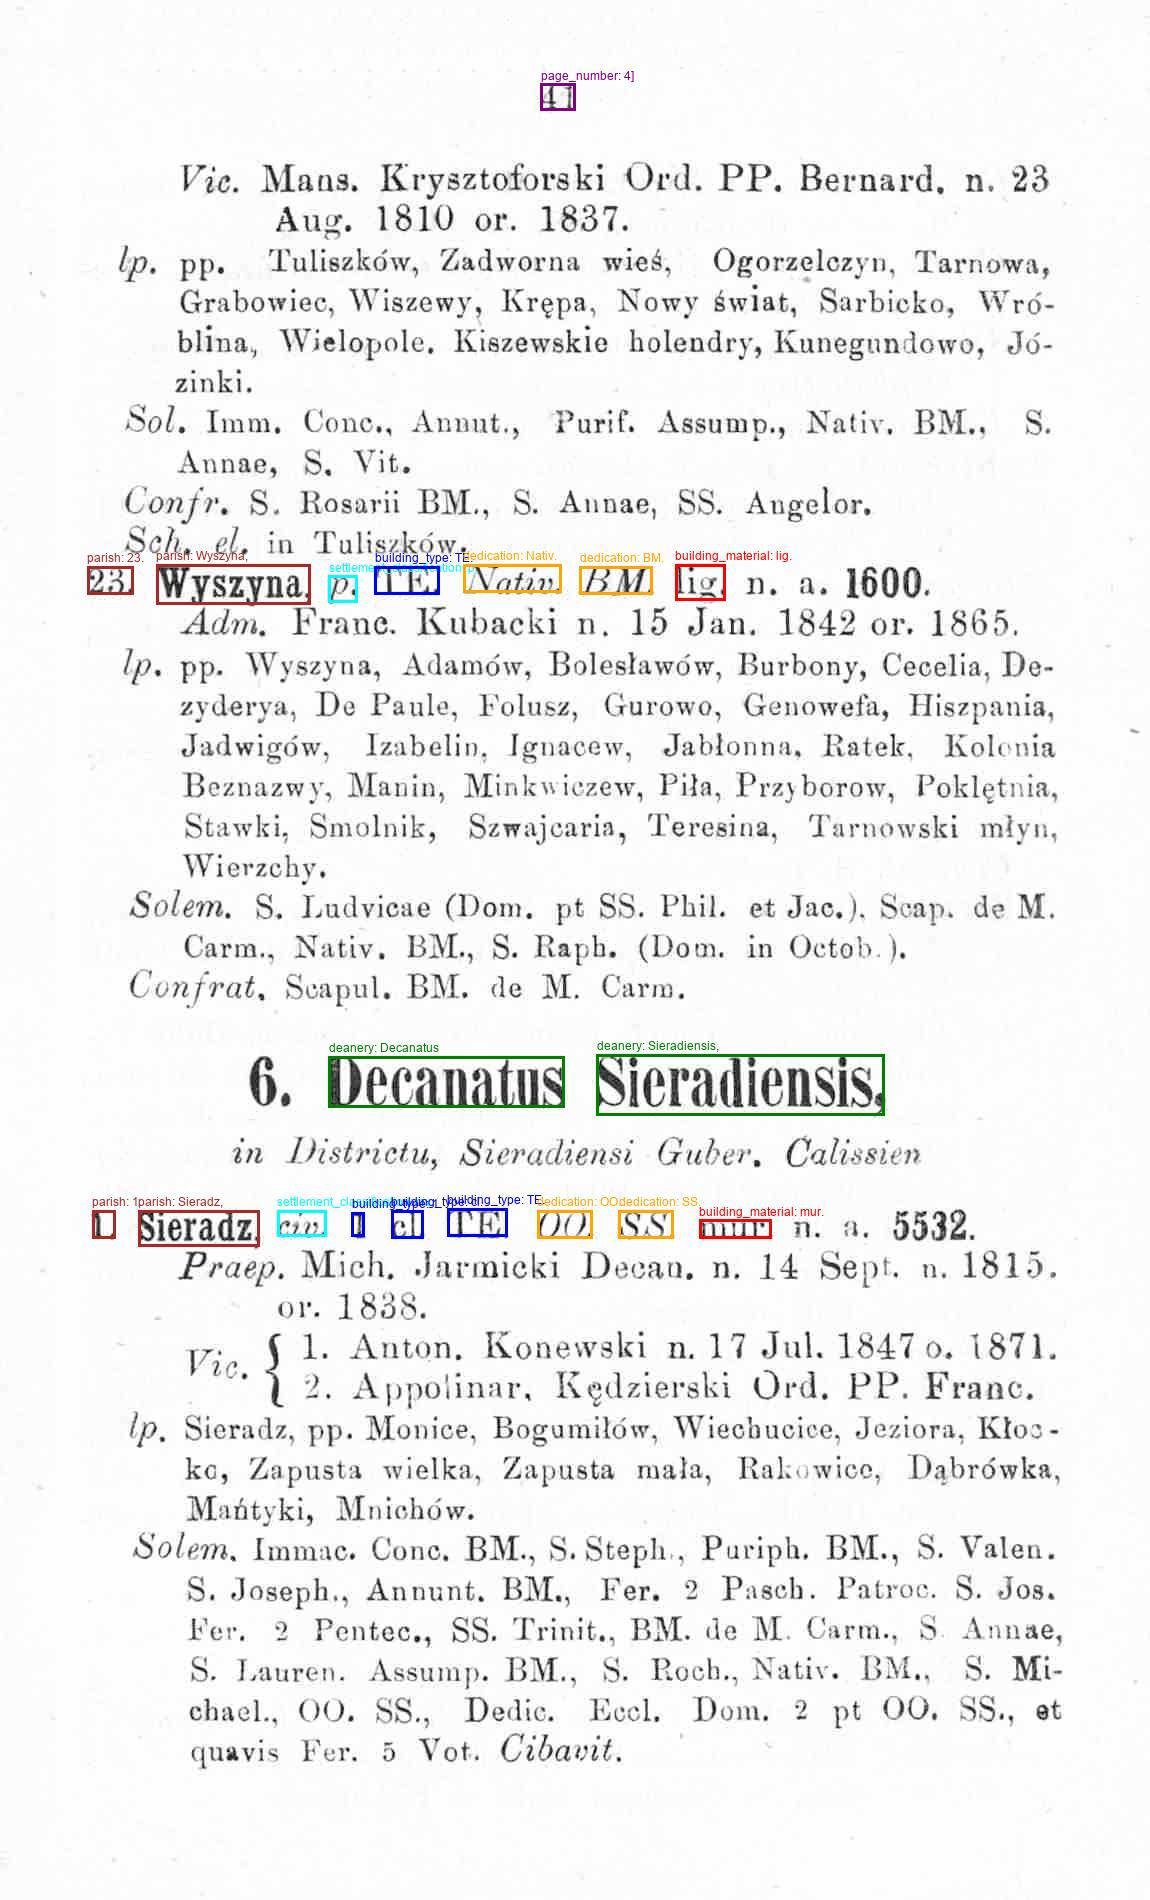
\includegraphics[width=0.72\textwidth]{layoutlmv3_predictions_ref.png}
\caption{Wizualizacja przykładowych predykcji modelu LayoutLMv3 na stronie schematyzmu. Kolorowe ramki pokazują tokeny przypisane przez model do klas używanych na etapie treningu, w tym numeru strony, nazwy parafii, dekanatu, wezwania, typu obiektu, materiału budowlanego oraz klasyfikacji miejscowości.}
\label{fig:layoutlmv3-predictions}
\end{figure}

\begin{figure}[htbp]
\centering
\begin{tikzpicture}[
    >=latex,
    node distance=0.6cm and 0.6cm,
    every node/.style={font=\footnotesize},
    block/.style={draw, rounded corners, fill=gray!10, text width=2.5cm, minimum height=1.5cm, align=center},
    issue/.style={draw, rounded corners, dashed, fill=red!8, text width=4.6cm, minimum height=1.2cm, align=center}
]
\node[block] (scan) {Obraz strony};
\node[block, right=of scan] (ocr) {OCR + boksy słów};
\node[block, right=of ocr] (lmv3) {LayoutLMv3};
\node[block, right=of lmv3] (entities) {Etykiety BIO / pola};
\node[issue, below=0.9cm of ocr, xshift=3.2cm] (issue) {Dobre wyniki lokalne, ale słaba generalizacja po dodaniu schematyzmów o innym układzie typograficznym.};
\draw[->, thick] (scan) -- (ocr);
\draw[->, thick] (ocr) -- (lmv3);
\draw[->, thick] (lmv3) -- (entities);
\draw[->, thick] (lmv3) -- (issue);
\end{tikzpicture}
\caption{Próba oparcia ekstrakcji na wytrenowanym modelu LayoutLMv3.}
\label{fig:layoutlmv3-approach}
\end{figure}

\subsection{Programistyczne przetwarzanie strona po stronie z własnymi promptami}\label{subsec:strona_bez_kontekstu}

Po doświadczeniach z gotowym interfejsem oraz z modelem dokumentowym zdecydowano się na zbudowanie własnego potoku programistycznego.
Dokument PDF dzielono na obrazy pojedynczych stron, a następnie dla każdej z nich wykonywano osobne wywołanie modelu wielomodalnego.
Kluczowa różnica polegała na tym, że zapytanie nie było już swobodną wiadomością wpisywaną w interfejs, lecz kontrolowaną konstrukcją złożoną z własnego promptu systemowego, własnego promptu użytkownika oraz oczekiwanego formatu odpowiedzi.
To podejście pozwoliło wymusić bardziej stabilny zwrot danych w postaci ustrukturyzowanej i znacząco poprawiło związek wyniku z konkretną stroną źródła.
Jednocześnie odsłoniło ono główny problem merytoryczny całego zadania: jeśli dekanat nie był jawnie widoczny na analizowanej stronie, model wciąż nie miał podstaw, aby poprawnie go odziedziczyć.
Schemat tego etapu pokazuje rys.~\ref{fig:custom-page-approach}.

\begin{figure}[htbp]
\centering
\begin{tikzpicture}[
    >=latex,
    node distance=0.6cm and 0.6cm,
    every node/.style={font=\footnotesize},
    block/.style={draw, rounded corners, fill=gray!10, text width=2.5cm, minimum height=1.5cm, align=center},
    issue/.style={draw, rounded corners, dashed, fill=red!8, text width=4.4cm, minimum height=1.2cm, align=center}
]
\node[block] (page) {Obraz jednej strony};
\node[block, right=of page] (prompt) {Własny system prompt + user prompt};
\node[block, right=of prompt] (llm) {Wywołanie Vision LLM};
\node[block, right=of llm] (json) {JSON strony};
\node[issue, below=0.9cm of prompt, xshift=3.1cm] (issue) {Lepsza kontrola formatu odpowiedzi, ale brak mechanizmu dziedziczenia dekanatu między stronami.};
\draw[->, thick] (page) -- (prompt);
\draw[->, thick] (prompt) -- (llm);
\draw[->, thick] (llm) -- (json);
\draw[->, thick] (llm) -- (issue);
\end{tikzpicture}
\caption{Programistyczne wywołanie modelu dla pojedynczej strony z użyciem własnych promptów.}
\label{fig:custom-page-approach}
\end{figure}

\subsection{Przetwarzanie sekwencyjne z propagacją kontekstu}\label{subsec:sekwencyjne_z_kontekstem}

Rozwiązanie przyjęte na ostatnim etapie eksperymentów zachowało zalety własnego potoku programistycznego, ale zostało uzupełnione o mechanizm propagacji stanu między kolejnymi stronami.
Po przetworzeniu każdej strony model zwraca, obok właściwych rekordów parafialnych, obiekt kontekstu zawierający aktualnie obowiązujący dekanat, numer ostatnio przetworzonej strony, streszczenie dotychczasowej zawartości dokumentu oraz opcjonalną adnotację sygnalizującą niską pewność odczytu.
Przy przetwarzaniu kolejnej strony obiekt ten jest włączany do treści następnego zapytania, dzięki czemu model otrzymuje informację pomocną przy dziedziczeniu przynależności dekanalnej nawet wówczas, gdy nagłówek dekanatu nie pojawia się na bieżącej stronie.
Własne prompty systemowy i użytkownika zostały na tym etapie dopracowane tak, aby precyzyjnie definiowały rolę modelu, zasady dziedziczenia dekanatu, reguły odczytu układów wielokolumnowych oraz oczekiwany format JSON.
Ważnym uzupełnieniem stało się także dołączanie tekstu OCR strony następnej, który pomaga domknąć wpisy urwane u dołu bieżącej karty.
Schemat wybranego rozwiązania pokazano na rys.~\ref{fig:sequential-context-approach}.

W praktyce system zarządza historią konwersacji na dwa sposoby.
W wariancie akumulacyjnym przechowywana jest pełna historia wymiany z modelem, z której usuwane są jedynie obrazy i tekst OCR kolejnych stron, aby ograniczyć objętość przy zachowaniu ciągłości merytorycznej.
W wariancie okna przesuwnego historia jest przycinana do ustalonej liczby ostatnich wymian, a długoterminowy kontekst przenoszony jest wyłącznie przez obiekt kontekstu.
To właśnie ten etap został przyjęty jako architektura rozwiązania końcowego, choć dalsza część artykułu pokazuje, że uzyskana skuteczność pozostała wyraźnie zróżnicowana między polami.

\begin{figure}[htbp]
\centering
\begin{tikzpicture}[
    scale=0.9,
    transform shape,
    >=latex,
    every node/.style={font=\footnotesize},
    page/.style={draw, rounded corners, fill=blue!8, text width=2.8cm, minimum height=1.4cm, align=center},
    process/.style={draw, rounded corners, fill=gray!10, text width=2.4cm, minimum height=1.2cm, align=center},
    json/.style={draw, rounded corners, fill=green!8, text width=1.8cm, minimum height=1.1cm, align=center},
    context/.style={draw, rounded corners, fill=yellow!15, text width=2.4cm, minimum height=1.1cm, align=center},
    carry/.style={->, thick, rounded corners=6pt},
    label/.style={font=\tiny, align=center, fill=white, inner sep=1.5pt}
]
\node[page] (pageN) at (0,0) {Strona $n$\\obraz + OCR};
\node[process] (procN) at (0,-2.0) {Własne prompty\\+ Vision LLM};
\node[json] (jsonN) at (-1.25,-4.0) {JSON\\strony $n$};
\node[context] (ctxN) at (1.50,-4.0) {\texttt{PageContext}$_n$};

\node[page] (pageN1) at (5.9,0) {Strona $n{+}1$\\obraz + OCR};
\node[process] (procN1) at (5.9,-2.0) {Własne prompty\\+ Vision LLM};
\node[json] (jsonN1) at (4.65,-4.0) {JSON\\strony $n{+}1$};
\node[context] (ctxN1) at (7.40,-4.0) {\texttt{PageContext}$_{n+1}$};

\node[page] (pageN2) at (11.8,0) {Strona $n{+}2$\\obraz + OCR};
\node[process] (procN2) at (11.8,-2.0) {Własne prompty\\+ Vision LLM};
\node[json] (jsonN2) at (10.55,-4.0) {JSON\\strony $n{+}2$};
\node[context] (ctxN2) at (13.30,-4.0) {\texttt{PageContext}$_{n+2}$};

\draw[->, thick] (pageN) -- (procN);
\draw[->, thick] (procN) -- (jsonN);
\draw[->, thick] (procN) -- (ctxN);

\draw[->, thick] (pageN1) -- (procN1);
\draw[->, thick] (procN1) -- (jsonN1);
\draw[->, thick] (procN1) -- (ctxN1);

\draw[->, thick] (pageN2) -- (procN2);
\draw[->, thick] (procN2) -- (jsonN2);
\draw[->, thick] (procN2) -- (ctxN2);

\draw[carry] (ctxN.north) to[out=70,in=250] node[midway, above, label] {kontekst dziedziczony\\przez stronę $n{+}1$} (pageN1.west);
\draw[carry] (ctxN1.north) to[out=70,in=250] node[midway, above, label] {kontekst dziedziczony\\przez stronę $n{+}2$} (pageN2.west);
\end{tikzpicture}
\caption{Rozwiązanie końcowe: sekwencyjne przetwarzanie stron $n$, $n{+}1$ i $n{+}2$, w którym każda odpowiedź generuje obiekt \texttt{PageContext} przekazywany do następnego kroku.}
\label{fig:sequential-context-approach}
\end{figure}


\section{Architektura hybrydowa: OCR, model dokumentowy i model wizyjny}\label{subsec:architektura}

Ostatecznie przyjęta metoda opiera się na trzech komponentach działających sekwencyjnie dla każdej strony.

Pierwszy stanowi optyczne rozpoznawanie znaków (OCR).
Początkowo wykorzystywano w tym celu silnik Tesseract, skonfigurowany do obsługi trzech alfabetów (łacińskiego, polskiego i rosyjskiego), który dostarcza surowy tekst strony wraz ze współrzędnymi każdego rozpoznanego słowa na obrazie \parencite{smith2007tesseract}.
Tesseract zwraca jednak jednorodny strumień tekstu, pozbawiony informacji o strukturze typograficznej oryginału: pogrubienia nagłówków dekanatów, tabelaryczne zestawienia danych parafialnych czy podziały na kolumny zostają utracone.
Tymczasem cechy te okazały się istotne zarówno dla poprawnej interpretacji źródła, jak i dla skuteczności dalszych etapów ekstrakcji.
Potrzeba ich zachowania skłoniła do zastosowania na etapie OCR również modelu wizyjnego (Vision LLM), który konwertuje skan strony na tekst w formacie Markdown wiernie odwzorowującym układ druku: nagłówki, pogrubienia, podziały na akapity, tabele i strukturę kolumnową.
Rozwiązanie to jest znacząco bardziej wymagające obliczeniowo od klasycznego OCR, lecz dostarcza reprezentację tekstową bogatszą i bliższą oryginałowi.
W ostatecznej wersji systemu Tesseract pozostaje w użyciu wyłącznie jako źródło współrzędnych słów niezbędnych dla modelu LayoutLMv3, natomiast tekst strony przekazywany do głównego modelu ekstrakcji pochodzi z OCR realizowanego przez model wizyjny.
Żaden z wyników OCR nie jest traktowany jako autorytatywny. Oba pełnią rolę pomocniczą wobec obrazu strony, który pozostaje pierwotnym źródłem informacji.

Drugim komponentem jest model LayoutLMv3 firmy Microsoft, wyspecjalizowany w rozumieniu układu dokumentów \parencite{huang2022layoutlmv3}.
W ramach projektu podjęto próbę wytrenowania tego modelu jako samodzielnego narzędzia ekstrakcji.
W tym celu postawiono instancję platformy Label Studio z dedykowanym backendem uczenia maszynowego, umożliwiającym wstępne adnotowanie stron za pomocą bieżącej wersji modelu i ich ręczną korektę przez anotatorów \parencite{labelstudio_ml_backend_2026}.
Zbiór treningowy objął dziesięć schematyzmów o zróżnicowanym charakterze, a model trenowano z użyciem notacji BIO na siedmiu klasach encji: parafia, dekanat, wezwanie, materiał budowlany, numer strony, typ obiektu oraz klasyfikacja miejscowości, stosując funkcję straty Focal Loss w celu zrównoważenia silnie nierównomiernego rozkładu klas \parencite{lin2017focal}.
Ostatnia z wymienionych klas nie została jednak wykorzystana w końcowym schemacie ekstrakcji przyjętym dla rozwiązania docelowego.
Wyniki na schematyzmach o układzie zbliżonym do danych treningowych były obiecujące, jednak dołączenie schematyzmów o odmiennej strukturze typograficznej powodowało wyraźny spadek jakości, ponieważ model nie generalizował dostatecznie dobrze na różnorodność formatów obecnych w korpusie.
Ponadto architektura LayoutLMv3 przetwarza każdą stronę niezależnie i nie oferuje mechanizmu propagacji kontekstu między stronami, co uniemożliwiało rozwiązanie problemu dziedziczenia przynależności dekanalnej opisanego w sekcji~\ref{sec:charakterystyka_zadania}.
Z tych powodów model ten nie został przyjęty jako samodzielne narzędzie ekstrakcji, lecz pełni rolę opcjonalnego generatora podpowiedzi: na podstawie obrazu strony i danych z Tesseracta oznacza poszczególne słowa etykietami pól, a wynik ten przekazywany jest do głównego modelu wizyjnego jako zestaw niepewnych sugestii wymagających weryfikacji na podstawie obrazu.

Trzeci i centralny komponent stanowi wielomodalny duży model językowy (\textit{Vision LLM}), zdolny do jednoczesnej analizy obrazu strony i towarzyszącego mu tekstu.
Model ten otrzymuje: obraz bieżącej strony jako pierwotne źródło informacji, tekst OCR bieżącej strony jako wsparcie, opcjonalne podpowiedzi z modelu LayoutLMv3, kontekst z poprzedniej strony oraz tekst OCR strony następnej, który służy uzupełnieniu wpisów rozpoczynających się na bieżącej stronie, lecz urwanych u jej dołu.
Na podstawie tych danych wejściowych model zwraca ustrukturyzowany obiekt JSON zawierający listę rekordów parafialnych i obiekt kontekstu do przekazania dalej.
Na poziomie operacyjnym oznacza to architekturę, w której surowy obraz strony trafia równolegle do dwóch torów OCR: klasycznego Tesseracta oraz OCR realizowanego przez model wizyjny.
Niezależnie od tego ten sam obraz wchodzi bezpośrednio do właściwego pakietu wejściowego modelu ekstrakcji, gdzie jest łączony z wynikami OCR, podpowiedziami LayoutLMv3 oraz dodatkowym kontekstem wielostronicowym.
Schemat tej architektury przedstawiono na rys.~\ref{fig:system-architecture}.

\begin{figure}[htbp]
\centering
\begin{tikzpicture}[
    scale=0.9,
    transform shape,
    >=latex,
    every node/.style={font=\footnotesize},
    source/.style={
        draw,
        rounded corners,
        fill=blue!8,
        text width=2.8cm,
        minimum height=1.35cm,
        align=center
    },
    aux/.style={
        draw,
        rounded corners,
        fill=gray!10,
        text width=3.0cm,
        minimum height=1.25cm,
        align=center
    },
    input/.style={
        draw,
        rounded corners,
        fill=yellow!15,
        text width=3.3cm,
        minimum height=1.35cm,
        align=center
    },
    stage/.style={
        draw,
        rounded corners,
        fill=orange!12,
        text width=3.3cm,
        minimum height=1.45cm,
        align=center
    },
    output/.style={
        draw,
        rounded corners,
        fill=green!10,
        text width=3.3cm,
        minimum height=1.45cm,
        align=center
    },
    arrow/.style={->, thick}
]

% Main flow
\node[source] (scan) at (4,0) {Obraz bieżącej\\strony};

\node[aux] (tesseract) at (4,1.8) {Tesseract OCR\\tekst + współrzędne słów};
\node[aux] (visionocr) at (4,-1.8) {Vision LLM OCR\\tekst strony w Markdown};

\node[input] (context) at (8,2.3)  {Dodatkowy kontekst\\poprzednia strona + OCR strony następnej};

\node[aux] (layoutlmv3) at (8,-2.3) {LayoutLMv3\\podpowiedzi pól};

\node[stage] (packet) at (9,0) {Pakiet wejściowy XML\\obraz + OCR + podpowiedzi + kontekst};

\node[stage] (llm) at (13,0) {Vision LLM\\właściwa ekstrakcja};

\node[output] (out) at (17,0) {JSON strony\\+ nowy PageContext};

% Arrows
\draw[arrow] (scan) -- (tesseract);
\draw[arrow] (scan) -- (visionocr);


\draw[arrow] (scan) -- (packet);
\draw[arrow] (tesseract) -- (packet);
\draw[arrow] (visionocr) -- (packet);
\draw[arrow] (context) -- (packet);
\draw[arrow] (layoutlmv3) -- (packet);

\draw[arrow] (packet) -- (llm);
\draw[arrow] (llm) -- (out);

\end{tikzpicture}
\caption{Pipeline ekstrakcji danych z pojedynczej strony dokumentu.}
\label{fig:system-architecture}
\end{figure}

Zachowanie modelu regulowane jest szczegółową instrukcją systemową o objętości ok.\ 350 wierszy, obejmującą: definicję roli, reguły ekstrakcji dla każdego pola, zasady odczytu układów jedno- i wielokolumnowych, reguły dziedziczenia kontekstu dekanalnego, dozwolone i zabronione korekty odczytu OCR oraz listę kontrolną jakości wynikowego obiektu JSON\@.
Istotne jest przy tym, że prompty nie miały postaci swobodnego opisu w języku naturalnym, lecz były organizowane w formacie XML-podobnym, z osobnymi blokami dla roli modelu, wejściowego kontekstu wielostronicowego, reguł ekstrakcji oraz schematu odpowiedzi.
Analogiczną strukturę miał prompt użytkownika, w którym osobnymi znacznikami przekazywano kontekst poprzedniej strony, podpowiedzi z LayoutLMv3 oraz tekst OCR strony bieżącej i następnej.
Instrukcję uzupełniają cztery przykłady wzorcowe (\textit{few-shot examples}), ilustrujące typowe scenariusze: stronę z nagłówkiem dekanatu, nagłówek pojawiający się w środku strony, wiele parafii na jednej stronie oraz stronę niezawierającą rekordów parafialnych.

\begin{figure}[htbp]
\centering
\begin{minipage}{0.93\textwidth}
\begin{lstlisting}
<SYSTEM_PROMPT>
  <MULTI_PAGE_CONTEXT>
    <SUMMARY_FIELD_IMPORTANCE>
      The `summary` field serves as a compressed memory
      of document progression.
    </SUMMARY_FIELD_IMPORTANCE>
  </MULTI_PAGE_CONTEXT>
  <VALUE_EXTRACTION_RULES>
    <DEANERY>
      If context provides active_deanery but no new heading
      appears: use inherited value
    </DEANERY>
  </VALUE_EXTRACTION_RULES>
  <OUTPUT_SCHEMA>
    ...
  </OUTPUT_SCHEMA>
</SYSTEM_PROMPT>
\end{lstlisting}
\end{minipage}
\caption{Fragment rzeczywistego promptu systemowego w formacie XML-podobnym. Osobne znaczniki porządkują kontekst wielostronicowy, reguły ekstrakcji oraz oczekiwany schemat odpowiedzi JSON.}
\label{fig:xml-prompt-fragment}
\end{figure}

\begin{figure}[htbp]
\centering
\begin{minipage}{0.93\textwidth}
\begin{lstlisting}
<USER_REQUEST>
  <PREVIOUS_PAGE_CONTEXT>
    <ACTIVE_DEANERY>Decanatus Wyszynensis</ACTIVE_DEANERY>
    <PREVIOUS_SUMMARY>Page 14: 3 parishes...</PREVIOUS_SUMMARY>
  </PREVIOUS_PAGE_CONTEXT>
  <MODEL_HINTS source="layoutlmv3">
    Suggestions from a smaller model...
  </MODEL_HINTS>
  <CURRENT_PAGE_TEXT>
    OCR text from the current page...
  </CURRENT_PAGE_TEXT>
  <NEXT_PAGE_TEXT>
    OCR text from the next page...
  </NEXT_PAGE_TEXT>
</USER_REQUEST>
\end{lstlisting}
\end{minipage}
\caption{Fragment promptu użytkownika. Osobne znaczniki przekazują kontekst odziedziczony z poprzedniej strony, podpowiedzi modelu LayoutLMv3 oraz pomocniczy tekst OCR dla strony bieżącej i następnej.}
\label{fig:xml-user-prompt-fragment}
\end{figure}

Rysunki~\ref{fig:sample-llm-input} i~\ref{fig:sample-llm-output} pokazują skrócony przykład rzeczywistego pakietu wejściowego oraz odpowiadającej mu odpowiedzi modelu dla strony otwierającej wykaz parafii w schematyzmie włocławskim z 1872 r.

\begin{figure}[htbp]
\centering
\begin{minipage}{0.93\textwidth}
\begin{lstlisting}
{
  "image_path": ".../e6857f7b020207a54378a0f014c1c470.jpeg",
  "previous_page_context": {
    "active_deanery": null,
    "summary": "Previous pages covered administrative lists
      and seminary details.",
    "last_page_number": "9"
  },
  "current_page_text": "10 ... Decanatus Vladislaviensis ...
    1. Włocławek ... Titul. Eccl. S. Joan. Bapt. murata ...",
  "next_page_text": "... continuation of clergy and localities ...",
  "model_hints": "parish: Włocławek; dedication: S. Joan. Bapt.;
    building_material: murata"
}
\end{lstlisting}
\end{minipage}
\caption{Skrócony przykład pakietu wejściowego przekazywanego do modelu dla pojedynczej strony. Obejmuje on obraz strony, kontekst odziedziczony z poprzedniej karty, tekst OCR oraz opcjonalne podpowiedzi modelu dokumentowego.}
\label{fig:sample-llm-input}
\end{figure}

\begin{figure}[htbp]
\centering
\begin{minipage}{0.93\textwidth}
\begin{lstlisting}
{
  "page_number": "10",
  "entries": [
    {
      "deanery": "Decanatus Vladislaviensis",
      "parish": "Włocławek",
      "dedication": "S. Joan. Bapt.",
      "building_material": "murata"
    }
  ],
  "context": {
    "summary": "Page 10: First page of parish records.
      Introduces Decanatus Vladislaviensis.",
    "note": null,
    "active_deanery": "Decanatus Vladislaviensis",
    "last_page_number": "10"
  }
}
\end{lstlisting}
\end{minipage}
\caption{Skrócony przykład odpowiedzi modelu dla tej samej strony. Oprócz właściwych rekordów zwracany jest także obiekt kontekstu wykorzystywany przy przetwarzaniu kolejnych stron.}
\label{fig:sample-llm-output}
\end{figure}

W toku eksperymentów przetestowano kilkanaście modeli wizyjnych różnych producentów.
Ostatecznie do systematycznej ewaluacji na pełnym korpusie wykorzystano model Gemini Flash firmy Google, który okazał się najbardziej obiecującym kompromisem jakości ekstrakcji, kosztu i szybkości przetwarzania \parencite{google_gemini_models_2026}.
Generowanie odpowiedzi odbywa się przy niskiej wartości parametru losowości (\textit{temperature} = 0,1), co ogranicza niedeterminizm wyników.
Jak pokazano w dalszych częściach artykułu, skuteczność tego rozwiązania pozostała jednak silnie zależna od rodzaju pola: najwyższa dla numeru strony i materiału budowlanego, a wyraźnie niższa dla dekanatu.

\section{Opis pakietu danych badawczych}\label{sec:pakiet_danych}

Korpus źródłowy obejmuje 72 schematyzmy diecezjalne z 23 diecezji polskich, reprezentujące dwa główne przedziały chronologiczne: lata sześćdziesiąte-osiemdziesiąte XIX wieku oraz lata trzydzieste XX wieku.
Każdy schematyzm został zdigitalizowany w postaci pliku PDF, a następnie podzielony na osobne obrazy stron w wysokiej rozdzielczości, stanowiące podstawowe dane wejściowe systemu ekstrakcji.

Dane referencyjne, względem których oceniana jest jakość automatycznej ekstrakcji, stanowi baza danych zbudowana ręcznie przez zespół historyków w ramach projektu <tutaj dac nazwe projektu>.
Dla każdego schematyzmu baza zawiera sekwencję rekordów parafialnych z wypełnionymi polami: dekanat, parafia, wezwanie i materiał budowlany, przyporządkowanymi do konkretnych stron źródłowych.
Zbiór ten, liczący łącznie ok. 35, 000 rekordów, pełni podwójną rolę: jest zarówno docelowym produktem prac dokumentacyjnych projektu głównego, jak i wzorcem (\textit{ground truth}) do ewaluacji narzędzia cyfrowego.
\section{Predykcja}\label{sec:predykcja}

Wynik automatycznej ekstrakcji dla każdego schematyzmu przyjmuje postać sekwencji rekordów o identycznej strukturze pól co dane referencyjne.
Ponieważ model ekstrakcji zwraca wartości w oryginalnej formie źródłowej (łacińskiej, rosyjskiej bądź niemieckiej), a baza referencyjna projektu głównego posługuje się polskimi odpowiednikami i skrótami, konieczny jest dodatkowy etap tłumaczenia, w dalszym ciągu określany jako \textit{parsowanie}.
Etap ten opiera się na trzech słownikach mapujących formy źródłowe na znormalizowane wartości polskie: dla materiału budowlanego (np.\ \textit{mur.}~$\rightarrow$~\textit{mr}, \textit{lign.}~$\rightarrow$~\textit{dr}), dla wezwań kościelnych (np.\ \textit{Assumptionis B.M.V.}~$\rightarrow$~\textit{Wniebowzięcie NMP}) oraz dla nazw dekanatów (np.\ \textit{Decanatus Gedanensis}~$\rightarrow$~\textit{Gdańsk}).
Aby uwzględnić warianty pisowni i drobne błędy w odczycie, dopasowanie w słownikach odbywa się z wykorzystaniem przybliżonego porównania łańcuchów z konfigurowalnym progiem tolerancji.
W rezultacie ewaluacja prowadzona jest dwutorowo: raz na poziomie formy źródłowej (\textit{source}), a raz na poziomie formy przetłumaczonej (\textit{parsed}), co pozwala oddzielnie mierzyć jakość samej ekstrakcji od jakości tłumaczenia na język docelowy bazy.
Porównanie obu sekwencji, referencyjnej i wygenerowanej, nie jest jednak trywialne: mogą się one różnić długością (model mógł pominąć pewne parafie lub wygenerować wpisy nieistniejące w źródle), a kolejność rekordów nie musi się pokrywać.
Problem ten rozwiązano za pomocą algorytmu węgierskiego, który znajduje optymalne przyporządkowanie parami między rekordami referencyjnymi a przewidywanymi, minimalizując łączną niepodobność.
Podobieństwo dwóch rekordów obliczane jest jako średnia ważona podobieństw poszczególnych pól, gdzie każde pole (dekanat, parafia, wezwanie, materiał budowlany) ma przypisaną wagę odzwierciedlającą jego znaczenie.
Podobieństwo pojedynczego pola mierzone jest znormalizowaną odległością Levenshteina po uprzednim sprowadzeniu obu wartości do formy porównywalnej: usunięciu znaków diakrytycznych, ujednoliceniu wielkości liter i normalizacji białych znaków.
Rekordy, których wzajemne podobieństwo nie przekracza ustalonego progu, nie są łączone w pary i trafiają odpowiednio do kategorii wpisów pominiętych (po stronie referencji) lub nadmiarowych (po stronie predykcji).


\section{Ewaluacja}\label{sec:ewaluacja}

Porównanie sekwencji referencyjnej i wygenerowanej rozpoczyna się od dopasowania rekordów za pomocą algorytmu węgierskiego \parencite{kuhn1955hungarian}.
Macierz podobieństwa budowana jest na podstawie ważonej zgodności pól rekordu, przy czym na etapie samego dopasowania implementacja korzysta ze znormalizowanych łańcuchów znaków i miary podobieństwa \texttt{SequenceMatcher} z biblioteki \texttt{difflib} \parencite{python_difflib_2026}.
Takie rozwiązanie pozwala zestawiać ze sobą sekwencje różniące się długością i kolejnością wpisów, a jednocześnie zachować próg jakości wymagany do uznania dwóch rekordów za odpowiadające sobie.

Po wykonaniu dopasowania obliczane są dwa typy ocen.
W wariancie \textit{source} dla każdego pola raportowane są miary podobieństwa tekstowego: średnia, minimum i maksimum.
W tym etapie wykorzystywany jest scorer oparty na znormalizowanym podobieństwie edycyjnym typu Levenshteina \parencite{wagner1974string}.
W wariancie \textit{parsed} ten sam typ porównania służy do wyznaczenia poprawności klasyfikacyjnej po przyłożeniu ustalonego progu zgodności.
Nie jest to jednak klasyczna macierz pomyłek budowana dla niezależnych obserwacji i zamkniętego zbioru etykiet.
Kategorie \textit{true positive}, \textit{false positive}, \textit{false negative} i \textit{true negative} wyznaczane są tu po wcześniejszym dopasowaniu rekordów, a następnie przez sprawdzenie, czy dana wartość pola została odtworzona w stopniu wystarczająco zgodnym z referencją.

Za trafienie (\textit{true positive}) uznaje się sytuację, w której zarówno wartość referencyjna, jak i przewidywana istnieją, a ich podobieństwo przekracza ustalony próg.
Wpis wygenerowany przez model, któremu nie odpowiada żadna wartość referencyjna, lub którego wartość odbiega od referencji poniżej progu, liczony jest jako błąd nadmiarowy (\textit{false positive}).
Analogicznie, wpis referencyjny bez odpowiadającej mu predykcji lub z predykcją poniżej progu stanowi pominięcie (\textit{false negative}).
W szczególności przypadek, w którym model zwrócił wartość dla pola, ale nie spełnia ona progu zgodności względem referencji, traktowany jest jednocześnie jako błąd nadmiarowy i pominięcie, ponieważ system wygenerował odpowiedź, lecz nie odtworzył poprawnej wartości.
Na tej podstawie wyznaczane są precyzja, czułość, dokładność oraz ich średnia harmoniczna (miara F1), oddzielnie dla każdego pola i dla każdego schematyzmu.

Wyniki ewaluacji eksportowane są w postaci arkuszy kalkulacyjnych, zawierających dla każdego schematyzmu zestawienie metryk per pole wraz z wierszem podsumowującym.
Nazwy plików wynikowych zawierają identyfikator użytego modelu oraz znacznik czasowy, co pozwala na systematyczne porównywanie kolejnych przebiegów eksperymentalnych.
Interpretacja tych metryk wymaga jednak rozbicia na poszczególne pola, ponieważ dalsza analiza jakościowa pokazuje wyraźne różnice między relatywnie łatwiejszym numerem strony i materiałem budowlanym a znacznie trudniejszym zadaniem poprawnego odziedziczenia dekanatu.


\printbibliography{}

% \tableofcontents

% Bibliografia

\end{document}
